\section{Auswertung}
\subsection{Überprüfung der Bragg Bedingung}
Die Messwerte zur Überprüfung der Bragg Bedingung befinden sich in Tabelle \ref{tab:tabe1},
welche sich, zusammen mit den anderen Messwerten, im Anhang befindet.
Sie sind in Abbildung \ref{fig:plot0} graphisch dargestellt.
\begin{figure}[H]
  \centering
  \includegraphics{plot0.pdf}
  \caption{Messwerte zur Überprüfung der Bragg-Bedingung}
  \label{fig:plot0}
\end{figure}

Hieraus lässt sich ein Maximum von 140 Impulsen pro s bei einem Winkel von 28,2°
ablesen.

\subsection{Emissionsspektrum der Cu-Röntgenröhre}
Die Messwerte des Emissionsspektrums sind in Tabelle \ref{tab:tabe2} abzulesen. In
Abbildung \ref{fig:plot1} sind sie zudem graphisch dargestellt.
\begin{figure}[H]
  \centering
  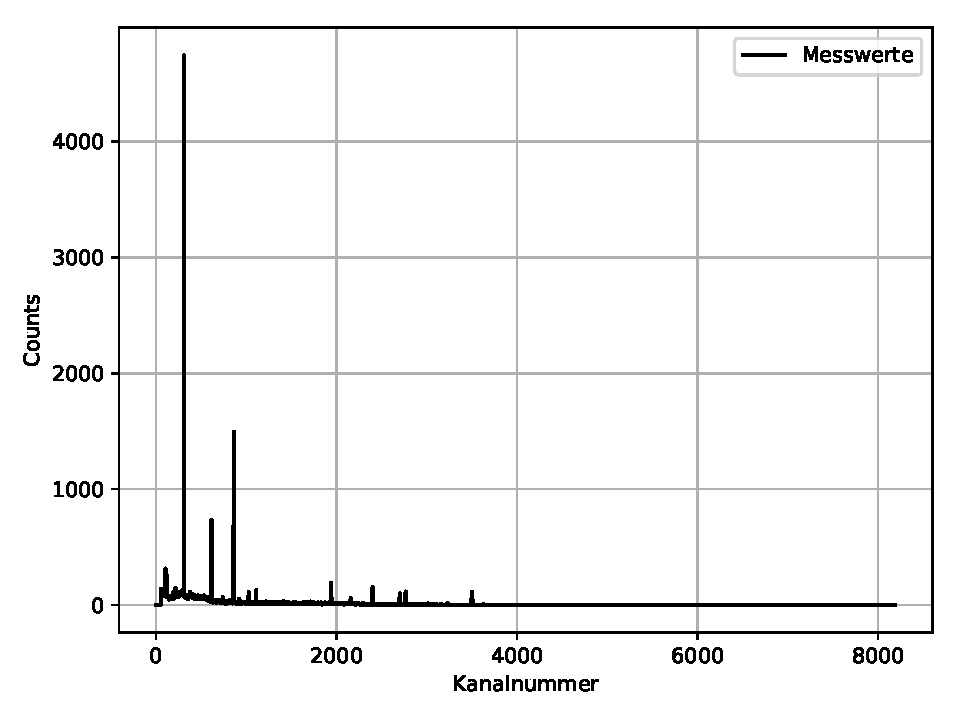
\includegraphics{plot1.pdf}
  \caption{Messwerte des Emissionsspektrums}
  \label{fig:plot1}
\end{figure}
Der Grenzwinkel beträgt hierbei etwa 10°, woraus sich nach Formel \ref{eqn:bragg} eine minimale
Wellenlänge von $ \SI{35.106}{\pico\meter}$ und eine maximale Energie von $\SI{5.658}{\femto\joule}$
bzw. $\SI{35.317}{\kilo \electronvolt}$ berechen lässt. Die Theoriewerte ergeben sich
aus Gleichung \ref{eqn:lamdbamin} zu einer minimalen Wellenlänge von $ \SI{35.424}{\pico\meter}$
und einer maximalen Energie von $\SI{5.608}{\femto\joule}$
bzw. $\SI{35}{\kilo \electronvolt}$
Durch die Formel
\begin{equation*}
  \frac{\lvert \text{Wert}_{\text{Theorie}}-\text{Wert}_{\text{Messung}}\rvert}{\text{Wert}_{\text{Theorie}}}
  \label{eqn:abw}
\end{equation*}
ergibt sich somit eine relative Abweichung von $0.9 \%$.

Aus Abbildung \ref{fig:plot1} lässt sich für die Halbwertsbreite der K$\alpha$-Linie
ein Wert von etwa $\Delta \theta$= 0,4° (zwischen 22,18° und 22.48°) ablesen und für die K$\beta$-Linie ein
Wert von etwa $\Delta \theta$= 0,35° (zwischen 19,85° und 20,20°).
Hieraus lässt sich durch $\Delta$E = $\text{E}_1$ - $\text{E}_2$
eine Auflösung von $\SI{0.14}{\kilo\electronvolt}$ (aus K$\alpha$) bzw. $\SI{0.15}{\kilo\electronvolt}$
(aus K$\beta$) berechnen.
Durch die Gleichung
\begin{equation}
  \bar{x} = \frac{1}{N} \sum_{i=1}^{N} x_i \: \:
  \label{eqn:mit}
\end{equation}
\noindent lässt sich der Mittelwert bilden, wobei der dazugehörige Fehler sich durch
\begin{equation}
  \increment \bar{x} = \frac{1}{\sqrt{N}} \sqrt{ \frac{1}{N-1} \sum_{i=1}^N
  (x_i - \bar{x})^2}
  \label{eqn:mitf}
\end{equation}
ergibt.
Somit ergibt sich also insgesamt eine Auflösung von $\SI{0.145(5)}{\kilo\electronvolt}$.\\
\\



%Die Energiedifferenz zwischen der K$\alpha$-Linie und der K$\beta$-Linie beträgt etwa $\SI{0.835}{\kilo\electronvolt}$.
%Aus der Gleichung \ref{eqn:???} ergibt sich hieraus eine Abschirmkonstante von
\noindent Die K$\alpha$-Linie liegt bei etwa 22,2 ° und die K$\beta$-Linie bei etwa 20,0°.
Das entspricht Energien von $\text{E}_{k\alpha} = \SI{8.146}{\kilo\electronvolt}$ und
$\text{E}_{k\beta} = \SI{9.000}{\kilo\electronvolt}$
Aus Gleichung \ref{eqn:k} ergeben sich somit Abschirmzahlen von
\begin{align*}
  \sigma_1 &= 3,275 \\
  \sigma_2 &= 13,151 \: . \\
\end{align*}

\subsection{Absorptionsspektren}
\subsubsection{Brom}
Die Messwerte des Absorptionsspektrums von Brom sind in Tabelle \ref{tab:tabe3} aufgeführt und
in Abbildung \ref{fig:brom} graphisch dargestellt.
\begin{figure}[H]
  \centering
  \includegraphics{Brom.pdf}
  \caption{Absorptionsspektrum von Brom}
  \label{fig:brom}
\end{figure}
Die K-Kante liegt hierbei bei einem Winkel von ungefähr 13,03°, welcher sich durch
das Ablesen des Graphen mittels Python ergibt. Hieraus ergibt sich nach Formel
\ref{eqn:bragg} eine Absorptionsenergie von $\SI{13.657}{\kilo\electronvolt}$. Durch Gleichung
\ref{eqn:abw} ergibt sich somit eine prozentuale Abweichung von 1,16 \%
zum Theoriewert aus der Vorbereitung.


Aus Gleichung \ref{eqn:Ebindung} lässt sich aus dieser Absorptionsenergie eine Abschirmkonstante
von 3,317 berechnen, wobei die relative Abweichung 5,23 \% beträgt.

\subsubsection{Strontium}
Die Messwerte des Absorptionsspektrums von Strontium sind in Tabelle \ref{tab:tabe4} aufgeführt und
in Abbildung \ref{fig:Strontium} graphisch dargestellt.
\begin{figure}[H]
  \centering
  \includegraphics{Strontium.pdf}
  \caption{Absorptionsspektrum von Strontium}
  \label{fig:Strontium}
\end{figure}
Die K-Kante liegt hierbei bei einem Winkel von etwa 10,85°. Nach analoger Rechnung zu Brom
ergibt sich für Strontium somit eine Absorptionsenergie von $\SI{16.352}{\kilo\electronvolt}$
(relative Abweichung: 1,57 \%) und eine Abschirmkonstante von 3,332 (relative Abweichung: 7,44 \%).

\subsubsection{Zink}
Die Messwerte des Absorptionsspektrums von Zink sind in Tabelle \ref{tab:tabe5} aufgeführt und
in Abbildung \ref{fig:Zink} graphisch dargestellt.
\begin{figure}[H]
  \centering
  \includegraphics{Zink.pdf}
  \caption{Absorptionsspektrum von Zink}
  \label{fig:Zink}
\end{figure}
Die K-Kante liegt hierbei bei einem Winkel von etwa 18,38°. Nach analoger Rechnung
ergibt sich für Zink somit eine Absorptionsenergie von $\SI{9.765}{\kilo\electronvolt}$
(relative Abweichung: 1,19 \%) und eine Abschirmkonstante von 3,210 (relative Abweichung: 4,75 \%).

\subsubsection{Zirkonium}
Die Messwerte des Absorptionsspektrums von Zirkonium sind in Tabelle \ref{tab:tabe6} aufgeführt und
in Abbildung \ref{fig:Zirkonium} graphisch dargestellt.
\begin{figure}[H]
  \centering
  \includegraphics{Zirkonium.pdf}
  \caption{Absorptionsspektrum von Zirkonium}
  \label{fig:Zirkonium}
\end{figure}
Die K-Kante liegt hierbei bei einem Winkel von etwa 9,68°. Nach analoger Rechnung
ergibt sich für Zirkonium somit eine Absorptionsenergie von $\SI{18.315}{\kilo\electronvolt}$
(relative Abweichung: 1,75 \%) und eine Abschirmkonstante von 3,309 (relative Abweichung: 8,59 \%).
\subsubsection{Moseleysches-Gesetz}
Zur Bestimmung der Rydbergkonstanten wird in Abbildung \ref{fig:plot7} die Wurzel der Energie
der K$\alpha$-Linie gegen die Kernladungszahl Z aufgetragen und eine lineare Ausgleichsrechnung
durchgeführt.
\begin{figure}[H]
  \centering
  \includegraphics{plot7.pdf}
  \caption{Lineare Ausgleichsrechnung der Wertepaare}
  \label{fig:plot7}
\end{figure}
Hieraus ergeben sich die Parameter
\begin{align*}
  a = (3,649 \pm 0,02) \frac{1}{\sqrt{eV}} \\
  b = (-10,7 \pm 0,6) \sqrt{eV} \: \: . \\
\end{align*}
Nach Gleichung \ref{eqn:Ebindung} beträgt die Steigung dieser
Geraden etwa $\sqrt{\text{R}_{\infty}}$,
wobei $\text{R}_{\infty}$ die gesuchte Rydbergenergie
bezeichnet, welche somit
\begin{align*}
  \text{R}_{\infty}= \SI{13.313}{\electronvolt}
\end{align*}
beträgt und eine relative Abweichung von 2,11 \% zum Theoriewert aufweist.
\subsubsection{Gold}
Die Messwerte des Absorptionsspektrums von Gold sind in Tabelle \ref{tab:tabe7} aufgeführt und
in Abbildung \ref{fig:Gold} graphisch dargestellt.
\begin{figure}[H]
  \centering
  \includegraphics{Gold.pdf}
  \caption{Absorptionsspektrum von Gold}
  \label{fig:Gold}
\end{figure}
Die beiden L-Kanten liegen bei $\theta_1$ = 12,9° und bei $\theta_2$ = 14,9°, was Energien
von $\text{E}_{1} = \SI{13.788}{\kilo\electronvolt}$ und
$\text{E}_{2} = \SI{11.971}{\kilo\electronvolt}$ entspricht, sodass die Energiedifferenz
$\Delta E_L = \SI{1.817}{\kilo\electronvolt}$ ist.
Aus Gleichung \ref{eqn:L} lässt sich hiermit eine Abschirmkonstante von
$\sigma_L = 3,556$ berechnen.
